Poniższy rozdział omawia implementację aplikacji służącej jako intranet dla firmy z sektora IT, opisane zostaną założenia oraz --wymagania stawanie dla strony serwerowej oraz dla klientów--. W rozdziale poruszone zostaną najistotniejsze oraz kluczowe elementy aplikacji. Aplikacja została napisana z wykorzystaniem frameworka Meteor.js. Część serwera jak i kliencka została za programowana z użyciem JavaScriptu. Warstwa prezentacji została napisana z użyciem HTML5, CSS3/less, Bootstrap oraz AdminLTE. Bazę danych dla aplikacji stanowi nierelacyjna baza danych MongoDB wraz z jej kliencką implementacją Minimongo.

\section{Założenia}
% założenia aplikacji intranet

Jak już wspomniono wcześniej do najważniejszych funkcjonalności aplikacji intranetowych zaliczamy dzielenie wiedzy oraz informacji, komunikację pomiędzy pracownikami danej organizacji oraz wspomaganie pracy zespołowej. W oparciu o ten najważniejsze funkcjonalności budowana aplikacja powinna spełniać następujące założenia:
\begin{itemize}
 \item tworzenie oraz rejestracja organizacji;
 \item tworzenie oraz rejestracja użytkowników;
 \item nazwa użytkownika oraz organizacji to jego emial;
 \item dodawanie utworzonego użytkownika do organizacji;
 \item tworzenie oraz rejestracja użytkowników z wykorzystaniem zaproszeń powiązanych z organizacją;
 \item organizacja w swoim zakresie, powinna posiadać główny zbiór artykułów --- główne wiki\footnote{Typ serwisu internetowego, w którym treść można tworzyć i zmieniać z poziomu przeglądarki internetowej, za pomocą języka znaczników lub edytora WYSIWYG. Strony wiki, ze względu na swoją specyfikę, są przede wszystkim wykorzystywane do pracy nad wspólnymi projektami, takimi jak repozytoria wiedzy na wybrany temat lub projekty różnych grup społecznych};
 \item główne wiki dla organizacji ma być one widoczne dla wszystkich użytkowników należących do danej organizacji; 
 \item główne wiki ma posiadać główną kategorię, której nie można usunąć;
 \item tworzenie, edycja, usuwanie kategorii artykułów w głównej wiki;
 \item tworzenie, edycja, usuwanie artykułów w głównej wiki; 
 \item artykuły mogą być dodawana do głównej kategorii wiki lub do utworzonych przez użytkownika kategorii;
 \item edycja oraz prezentacja artykułów na obsługiwać język znaczników \emph{markdown}\footnote{Język znaczników przeznaczony do formatowania tekstu zaprojektowany przez Johna Grubera i Aarona Swartza. Został stworzony w celu jak najbardziej uproszczenia tworzenia i formatowania tekstu. Markdown został oryginalnie stworzony w Perlu, później dostępny w wielu innych. Jest rozpowszechniany na licencji BSD i jest dostępny jako wtyczka do kilku systemów zarządzania treścią.} w szczególności jego implementację \textit{GitHub Flavored Markdown} --- GFM;
 \item artykuły mogą mieć stan opublikowany oraz do publikacji;
 \item użytkownik nie będący twórcą danej organizacji ma dostęp tylko do artykułów opublikowanych przez innych użytkowników oraz do wszystkich swoich artykułów niezależnie od ich stanu;
 \item organizacja ma dostęp w swoim zakresie do wszystkich artykułów, wszystkich użytkowników należących do danej organizacji niezależnie od stanu ich publikacji;
 \item kategoria, w której są artykuły nie może zostać usunięta;
 \item artykuł może należeć tylko do jednej kategorii;
 \item użytkownik w swoim zakresie posiada główną wiki;
 \item główna wiki dla użytkownika jest widoczna tylko dla niego w jego zakresie;
 \item główna wiki dla użytkownika ma takie same funkcjonalności jak główna wiki dla organizacji;
 \item prezentacja, tworzenie, edycja oraz usuwanie artykułów dla głównego wiki dla użytkownika ma spełniać opisane cechy jak dla artykułów dla organizacji; 
 \item użytkownicy mogą zmieniać zakres w pomiędzy zakresami organizacji, do których należą i swoim zakresem;
 \item organizacja oraz użytkownicy mogą tworzyć, usuwać projekty w swoich zakresach lub zakresach, do których należą;
 \item projekty powinny posiadać stronę z podsumowaniem;
 \item projekty powinny posiadać niezależne wiki;
 \item projekty powinny mieć możliwością dodawania --- zapraszanie --- użytkowników oraz ich usuwanie;
 \item wiki dla projektów ma mieć te same cechy jak główne wiki;
 \item projekty powinny posiadać możliwość komunikacji pomiędzy użytkownikami przynależącymi do danego projektu;
 \item twórca projektu może dodawać oraz usuwać użytkowników, którzy mają do niego dostęp;
 \item użytkownicy widzą tylko projekty, do których zostali zaproszeni;
 \item organizacja ma dostęp do wszystkich projektów utworzonych w jej zakresie;
 \item komunikacja w obrębie projektu mam mieć możliwość dodania wiadomości wraz z jej tytułem oraz możliwością dodana komentarzy;
 \item wysyłanie zaproszeń do projektów oraz organizacji --- jeżeli użytkownik z podanym adresem email istnieje w systemie ma być automatycznie dodany do projektu lub organizacji;
 \item aplikacja ma być dostępna na wszystkich znaczących platformach oraz jak największej ilości urządzeń.
\end{itemize} 

\section{Wymagania}
% tu zobaczym czy to będzie opis ogólnie dlaczego został wybarny meteor a nie inne rozwiązanie - można wspomnieć o szybkości kodowania oraz że tematyka nie stoi w sprzeczości z frameworkiem oraz samym mongo 

Niezależność od platformy oraz dostępność na jak największej ilości urządzeń narzuciła wybór typu aplikacji. Budowana aplikacja będzie typu sieciowego. Klienci będą uzyskiwać do niej dostęp poprzez przeglądarki internetowe kontaktując się z serwerem, na którym będzie dostępna budowana aplikacja. 

W oparciu o założenia jakie ma spełniać aplikacja \emph{Intranet} oraz o obecne trendy w rozwoju aplikacji sieciowych do budowy aplikacji został wybrany framework Meteor.js, a jako język programowania JavaScript. Wybór tych technologii był podyktowany także szybkością oraz prostotą budowania aplikacji. Meteor.js używa JavaScriptu zarówno po stornie klienta oraz serwera co skraca czas nauki samego framework'a eliminując potrzebę nauki dodatkowego języka programowania. Tematyka oraz założenia projektu nie stanowią problemu dla przyjętego przez framework Meteor.js nierelacyjnego rozwiązania bazodanowego. Aplikacja nie posiada krytycznych elementów takich jak transakcje finansowe, zamówienia oraz innych elementów wymagających transakcji operacji na całej bazie danych. Dane są typowo informacyjne w związku z tym wykorzystanie bazy MongoDB nie stanowi żadnego zagrożenia dla użytkowników oraz samej aplikacji.

Aplikacja ma być dostępna na wszystkich znaczących platformach oraz jak największej ilości urządzeń. Aby to zapewnić w warstwie prezentacji wykorzystano HTML5, CSS3 wraz z kompilatorem less oraz domyślnie wykorzystywaną przez Meteor.js bibliotekę JQuery. W celu zachowania responsywności interfejsu użytkownika wykorzystano szablon AdminLTE, który oparty jest o framework Bootstrap. Wykorzystanie Bootstrapa dostarcza prosty oraz szybki sposób na dostosowanie układu i wyglądu interfejsu użytkownika w zależności od używanego przez niego urządzenia. Rozwiązanie to znaczenie zwiększa użyteczność aplikacji podczas używania urządzeń o różnych wielkościach oraz rozdzielczościach ekranu. 

\section{Struktura aplikacji}
%   nie zapomnieć o katalogu .meteor

Aplikacje napisane z wykorzystaniem frameworka Meteor.js to zestaw plików JavaScript, które działają w przeglądarce internetowej i w kontenerze Node.js po stronie serwera, i innych plików pomocniczych takich jak szablony HTML, kaskadowe arkusze stylów oraz statycznych zasobów. Meteor.js automatycznie pakuje oraz zajmuję się przesyłaniem tych różnych elementów. Framework jest dość elastyczny jeżeli chodzi o strukturę katalogów w jakiej będą umieszczone poszczególne elementy aplikacji. Nazwy plików jaki i katalogów mogą mieć wpływ na to w jakiej kolejności są one ładowane oraz gdzie są one ładowane. Meteor.js niektóre katalogi traktuje w specjalny sposób.

Katalogi o nazwie \verb|client| nie są ładowane po stronie serwera. Wszystkie zasoby znajdujące się w tym katalogu gdy aplikacja nie jest uruchomiona w trybie produkcyjnym są łączone oraz minimalizowane. W trybie developerskim plik JavaScript oraz CSS nie są minimalizowane aby ułatwić znajdowanie błędów w aplikacji. Jednakże pliki CSS nadal są łączone w jeden plik. Pliki HTML po stronie klienta są skanowane w poszukiwaniu trzech elementów najwyższego poziomu \verb|<head>|, \verb|<body>|, \verb|<template>|. Elementy head oraz body łączone są w jeden element i następnie przesyłane do klienta podczas pierwszego ładowania strony.

Zasoby znajdujące się w katalogach o nazwie \verb|server| nie są ładowane po stronie klienta. Krytyczne oraz wrażliwe elementy aplikacji takie jak zarządzenia hasłami, proces autoryzacji powinny znajdować się w tych katalogach. Meteor zbiera wszystkie pliki JavaScript za wyjątkiem tych znajdujących się w katalogach \verb|public|, \verb|client| i \verb|private| oraz ich podkatalogach i ładuje je do instancje Node.js znajdującej się na serwerze. Kod na serwerze nie jest uruchamiany jako kod asynchroniczny typowy dla aplikacji opartych o Node.js. Meteor uruchamia kod pojedynczy wątek na żądanie

Wszystkie pliki znajdujące w katalogu \verb|public| najwyższego poziomu serwowane są dla klientów takim jakimi są. Jest to właściwe miejsce dla plików takich jak \verb|favicon.ico|, \verb|robots.txt| oraz innych podobnych plików.

Pliki znajdujące się w katalogu najwyższego poziomu o nazwie \verb|private| dostępne są tylko po stronie serwera z wykorzystaniem API \verb|Assets|. Katalog ten przeznaczony jest dla takich plików jak prywatne dane oraz plików, które nie mają być dostępne z zewnątrz.

Podczas ładowanie plików przez Meteor.js obowiązują następujące reguły:
\begin{enumerate}
 \item szablony HTML ładowane są zawsze jako pierwsze;
 \item pliki zaczynające się na \verb|main.| ładowane są zawsze jako ostanie;
 \item następnie ładowane są pliki znajdujące się w jakimkolwiek katalogu \verb|lib/|;
 \item następnie ładowane są plik z głębszą ścieżką;
 \item następnie pliki ładowane są w kolejności alfabetycznej uwzględniającej całą ścieżkę katalogów.
\end{enumerate}


Wszystkie pliki JavaScript nie znajdujące się w specjalnych katalogach ładowane są zarówno po stronie klienta jaki i serwera. Jest to dobre miejsce na definicje modeli oraz innych funkcji, które mają być dostępne zarówno dla klienta jak i serwera. Meteor.js dostarcza zmienne \verb|Meteor.isClient| oraz \verb|Meteor.isServer|, które można użyć do zmiany zachowania w zależności czy kod jest uruchomiony na serwerze czy kliencie. Pliki CSS oraz HTML poza specjalnymi katalogami ładowane są tylko po stornie klienta i nie mogą zostać użyte po stronie serwera.

\begin{figure}[h]
%   \centering
\dirtree{%
.1 intranet.
.2 apps.
.3 app.
.3 invitation.
.3 mainDash.
.3 projects.
.3 users.
.3 wiki.
.2 private.
.3 subList.
.2 public.
.3 favicon.ico.
.3 square.png.
.3 square@2x.png.
.2 server.
.3 config.
.4 developConfig.json.
.4 exampleConfig.json.
.4 serverConfig.json.
.3 migrations.js.
.3 startUp.js.
}
%     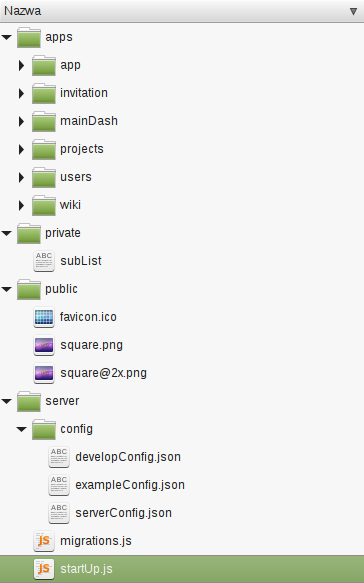
\includegraphics[width=0.5\textwidth]{ch03/intranet_005.png}
  \caption{Główny katalog aplikacji \emph{Intranet}}
  \label{fig:app_main_structure}
\end{figure}

Rysunek \ref{fig:app_main_structure} przedstawia główny katalog aplikacji \emph{Intranet}. Skład się on z następujących podkatalogów: \verb|apps|, \verb|private|, \verb|public|, \verb|server|. W katalogu \verb|apps| znajdują się poszczególne moduły aplikacji. Katalog \verb|private| zawiera zasoby nie dostępne z zewnątrz, znajduje się w nim opis subskrypcji wykorzystywanych przez aplikację. Katalog \verb|public| zawiera pliki graficzne używane przez aplikację. W katalogu \verb|server| znajduje się plik odpowiedzialny za migrację \verb|migrations.js| oraz plik \verb|startUp.js| zawierający kod uruchamiany na samym początku startu strony serwerowej. W podkatalogu \verb|config| zanajdują się pliki konfiguracyjne zapisane w postaci JSON. Plik \verb|developConfig.json| używany jest podczas pracy rozwojowych nad aplikacją. Plik \verb|serverConfig.json| używany jest w środowisku produkcyjnym.

Katalog \verb|apps| zawiera poszczególne moduły aplikacji. Podkatalog \verb|app| zawiera kod wykorzystywany w całej aplikacji, konfigurację używanych pluginów, globalne definicje \textit{helperów} --- funkcji pomocniczych używanych w szablonach HTML, pliki CSS wspólne dla całej aplikacji, pomocnicze szablony HTML oraz rozszerzenie wbudowanego obiektu szablonu o nową właściwość \verb|parentTemplate|.

\begin{figure}[h]
%   \centering
\dirtree{%
.1 intranet.
.2 apps.
.3 projects.
.4 client.
.5 addProjectForm.html.      
.5 addTalk.html.             
.5 addTalk.js.               
.5 projectAddUserForm.html.  
.5 projectAddUserForm.js.    
.5 projectTalks.js.
.5 projectMain.html.   
.5 projectMain.js.  
.5 projectRoutes.js. 
.5 projectTalks.html.
.5 styles.
.6 projet.less.
.5 talkElement.html.
.5 talkElement.js.
.4 lib.
.5 forms.js.  
.5 project.js.  
.5 projectsMethodes.js.  
.5 talks.js.
.4 server.
.5 projectPub.js.
.5 talksPub.js.
}
%     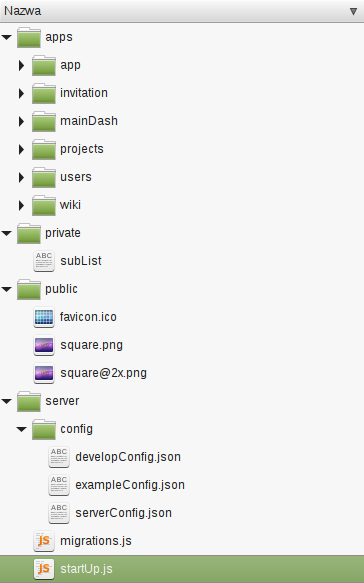
\includegraphics[width=0.5\textwidth]{ch03/intranet_005.png}
  \caption{Struktura przykładowego modułu \emph{projects}}
  \label{fig:app_project_structure}
\end{figure}

Rysunek \ref{fig:app_project_structure} przedstawia strukturę modułu \emph{projects} --- projekty. Widać w niej charakterystyczny podział aplikacji Meteor.js z wykorzystaniem katalogów specjalnych \verb|client| oraz \verb|server|. Katalog \verb|lib| zawiera kod wykorzystywany zarówno po stronie serwera jaki i klienta. Pliki zawarte w tym katalogu muszą zostać załadowane wcześniej niż kod znajdujący się w katalogach specjalnych. Kod ten zawiera definicje kolekcji projekty -- \verb|project.js| i konwersacji -- \verb|talks.js|, metody odpowiedzialne za operacje na danych w kolekcjach -- \verb|projectsMethodes.js| oraz definicje używanych przez moduł formularzy -- \verb|forms.js|. W katalogu \verb|client| znajdują się poszczególne widoki używane przez moduł oraz szablony poszczególnych elementów włączane przez inne szablony podczas renderowania ich zawartości. W pliku \verb|projectRoutes.js| zdefiniowane są trasy --- \textit{routing} --- dla modułu. Strona serwerowa składa się z dwu plików, które zawierają publikacje dla kolekcji jakich dostarcza moduł. Publikacje mogą być używane także poza modułem, w którym zostały zdefiniowane. Podkatalog \verb|styles| katalogu \verb|client| zawiera plik dynamicznego arkusza stylów less -- \verb|project.less|.

\section{Wspólna część dla strony serwerowej oraz klienckiej}

\subsection{Kolekcje} 
Dane, w bazie danych, wykorzystywane przez aplikację przechowane są w postaci dokumentów te natomiast grupowe są w logiczne zbiory nazywane kolekcjami. Klient oraz serwer używają tego samego API do dostępu do bazy danych. Klasa \verb|Mongo.Collection| używana jest do definiowania oraz manipulowania kolekcjami. Listing \ref{lst:project_coll} przedstawia sposób definicji kolekcji dla projektów --- \verb|Project|. Definicja jest umieszczona w katalogu \verb|lib| modułu \verb|projects|, który ładowany jest po stronie klienta jak i serwera przed plikami znajdującymi się w katalogach \verb|client| oraz \verb|server|. Tak zdefiniowaną kolekcję możemy używać po stronie serwera jak i klienta. 
\begin{js}[caption={{Definicja kolekcji dla projektów \textit{Project}}},label={lst:project_coll}]
Project = new Meteor.Collection('project');
\end{js}

Wykorzystując dodatkowy pakiet \verb|collection-hooks|\footnote{https://github.com/matb33/meteor-collection-hooks} możemy rozszerzyć klasę \linebreak \verb|Mongo.Collection| o dodatkowe właściwości dla operacji dodawania, modyfikowania oraz usuwania dokumentów w kolekcji wykonywane przed --- \verb|before| oraz po --- \verb|after| wykonaniu tych operacji. Przykładowe zastosowanie przedstawia listing \ref{lst:project_coll_hooks}. Rozszerzeniu ulegają operacje dodawania oraz modyfikacji. Przed wykonaniem operacji dodawania (\verb|insert|) dokumentu do kolekcji dodawane jest pole \verb|createdAt| z wartością ustawianą na dzisiejszą datę. Przed wykonywaniem operacji aktualizacji (\verb|update|) do modyfikatora jaki zostanie użyty podczas operacji aktualizacji dokumentu dodawane są pola \verb|modifiedAt| z wartością ustawioną na dzisiejszą datę oraz pole \verb|modifiedBy| z wartością jednoznacznie identyfikującą dokument użytkownika tak zwane \verb|_id| dokumentu.
Linia 12 listingu \ref{lst:project_coll_hooks} przedstawia użycie operatora \textit{lub} -- \verb|||| -- do przypisywania zmiennym, w tym przypadku argumentowi funkcji, wartości. Jeżeli argument ma wartość jego wartość się nie zmienia --- ulega ponownemu przypisaniu. Jeżeli natomiast wartość argumentu jest niezdefiniowana (\verb|undefined|) argumentowi przypisany zostanie pusty obiekt --- wyrażenie \verb|{}| jest literałem nowego obiektu. 
\begin{js}[caption={{Rozszerzanie kolekcji \textit{Project} o dodatkowe właściwości}},label={lst:project_coll_hooks}]
Project.before.insert(function (userId, doc) {
    "use strict";
    
    let createDate = new Date();
    doc.createdAt = createDate;
});

Project.before.update(function (userId, doc, fieldNames, modifier, options) {
    "use strict";
    
    let modDate = new Date();
    modifier.$set = modifier.$set || {};
    modifier.$set.modifiedAt = modDate;
    modifier.$set.modifiedBy = userId
});
\end{js}

\subsection{Metody}
Meteor.js oferuje mechanizm zdalnie wywoływanych metod. Klient może wywołać zdefiniowane metody zdalnie na serwerze. Metody są definiowane przez wywołanie \verb|Meteor.methods|. Wywołanie \verb|Meteor.methods| po stornie serwera tworzy funkcje, które mogą zostać zdalnie wywoływane przez klienta. Funkcje takie powinny zwracać wartość, która może zostać sparsowana do obiektu \textit{EJSON} lub zwracać błąd. Natomiast wywołanie \verb|methods| po stornie klienta definiuje funkcje typu \textit{stub} --- funkcja symulująca zachowanie metody o takiej samej nazwie  zdefiniowanej na serwerze. Jeżeli \textit{stub} zostanie zdefiniowany a klient wywoła metodę z nim powiązaną \textit{stub} zostanie wywołany równolegle. Po stronie klienta wartość zwracana przez \textit{stub} jest ignorowana. Funkcje \verb|stub| są uruchamiane dla ich skutków ubocznych --- ich celem jest symulacja wyników funkcji wywoływanych na serwerze bez konieczności oczekiwania na ich ukończenie oraz przesłanie ich wyniku z serwera.

\begin{js}[caption={{Wywołanie \textit{Meteor.methods} oraz definiowanie metod}},label={lst:projects_methods}]
Meteor.methods({
    removeUserFromProject (data) {
        check(data, {
            userId: String,
            projectId: String
        });
        
        let project = Project.findOne(data.projectId);
        if (Meteor.isServer) {
            
            if (!project || (!_.includes(project.secure.allowedUsers, this.userId) && project.secure.admin.id !== this.userId) ) {
                console.log('cant delete');
                throw new Meteor.Error(403, "Can't remove user from project");
            }
            Project.update({_id: project._id}, {$pull :{"secure.allowedUsers": data.userId, allowedUsers: data.userId}});
            return true;
        }


    },
    ...$
})

\end{js}
Wykorzystując \verb|Meteor.isServer| oraz \verb|Meteor.isClient| możemy rozdzielić kod metod na część wykonywaną tylko na serwerze, kliencie lub wspólnie dla obu przypadków. Definiując metody w części wspólnej dla serwera oraz klienta z wykorzystaniem powyższych elementów API możemy pominąć definiowanie \textit{stubów} dla metod po stronie klienta. Listing \ref{lst:projects_methods} przedstawia  tak zdefiniowaną metodę umieszczoną w  pliku \verb|projectsMethodes.js| znajdującym się w katalogu \verb|lib|. Metody mogą przyjmować argumenty. Do sprawdzenia poprawność argumentów metody można skorzystać z funkcji sprawdzających wzorce takich jak \verb|check| oraz \verb|Match.test|. Funkcje te dostarczane są przez pakiet \verb|check|. Listing przedstawia usuwanie użytkownika z projektu. Linia 15 przedstawia aktualizację dokumentu w kolekcji \verb|Project| o podanym \verb|_id|. Z tablicy \verb|allowedUsers| usuwany jest ciąg znaków zawierających id danego użytkownika przekazane do metody w argumencie \verb|data|. Pierwszym atrybutem przejmowanym przez metodę \verb|update| wykonywaną na rzecz kolekcji to selektor określający jaki dokument lub dokumenty mają zostać zmodyfikowane. Drugi argument to modyfikator określający sposób modyfikacji danego dokumentu. 

\section{Cześć serwerowa}
  \subsection{Baza danych}
  \subsubsection{Relacje}
Jako już wspomniano jako bazę danych wykorzystano MongoDB. Jest to baza nierelacyjna zorientowana na dokumenty, które logicznie grupowane są w kolekcje. Struktura dokumentów jest bardzo elastyczna a same kolekcje dokumentów nie narzucają jej. Aby odwzorować relacje pomiędzy dokumentami możemy użyć następujących wzorców: dokumenty wbudowane lub referencji.\newline 
Wzorzec dokumentów wbudowanych polega na dodaniu całego dokumentu od jakiego się odnosimy jako pola w innym dokumencie. Tak dodany dokument będzie odpowiadał relacji jeden do jednego. Listing \ref{lst:mongo_embeded_oto} przedstawia dwa dokumenty. Pierwszy reprezentuje osobę, drugi reprezentuje adres. Po dodaniu pola \verb|address| i przeniesieniu do niego całego dokumentu adresu uzyskujemy relację jeden do jednego z wykorzystaniem wzorca wbudowanych dokumentów. Wadą tego rozwiązania jest powielanie danych w bazie, zaletą natomiast to, że chcąc odczytać adres danej osoby pobieramy z bazy tylko jeden rekord.
\begin{js}[caption={{Dokumenty wbudowane -- relacja jeden do jednego}},label={lst:mongo_embeded_oto}]
// Dokumenty przed utworzeniem relacji
{
   _id: "joe",
   name: "Joe Bookreader"
}

{
   patron_id: "joe",
   street: "123 Fake Street",
   city: "Faketon",
   state: "MA",
   zip: "12345"
}

// Wzorzec dokumenty wbudowane relacja jeden do jednego

{
   _id: "joe",
   name: "Joe Bookreader",
   address: {
              street: "123 Fake Street",
              city: "Faketon",
              state: "MA",
              zip: "12345"
            }
}
\end{js}
Następny listing (\ref{lst:mongo_embeded_otm}) przedstawia wykorzystanie tego samego wzorca w celu uzyskania relacji jeden do wielu. Jak widać na listingu pole \verb|address| ma postać tablicy złożonej z dokumentów. 

\begin{js}[caption={{Dokumenty wbudowane -- relacja jeden do wielu}},label={lst:mongo_embeded_otm}]
{
   _id: "joe",
   name: "Joe Bookreader",
   addresses: [
                {
                  street: "123 Fake Street",
                  city: "Faketon",
                  state: "MA",
                  zip: "12345"
                },
                {
                  street: "1 Some Other Street",
                  city: "Boston",
                  state: "MA",
                  zip: "12345"
                }
              ]
}
\end{js}

Wzorzec referencji unikamy powielania danych poprzez podanie referencji do innego dokumentu w innej lub tej samej kolekcji. Referencją najczęściej jest  \verb|_id| dokumentu. Wadą tego wzorca jest konieczność pobierania kolejnych dokumentów z bazy w celu odczytania danych z dokumentu powiązanego. Wykorzystując ten wzorzec otrzymujemy relację jeden do wielu. Listing \ref{lst:mongo_ref} przedstawia wykorzystaniem podlegającej zmianie oraz rosnącej tablicy z \verb|_id| poszczególnych dokumentów.
\begin{js}[caption={{Referencje (tablica) -- relacja jeden do wielu}},label={lst:mongo_ref}]
{
   name: "O'Reilly Media",
   founded: 1980,
   location: "CA",
   books: [12346789, 234567890, ...] // _id of books for this publisher
}

{
    _id: 123456789,
    title: "MongoDB: The Definitive Guide",
    author: [ "Kristina Chodorow", "Mike Dirolf" ],
    published_date: ISODate("2010-09-24"),
    pages: 216,
    language: "English"
}

{
   _id: 234567890,
   title: "50 Tips and Tricks for MongoDB Developer",
   author: "Kristina Chodorow",
   published_date: ISODate("2011-05-06"),
   pages: 68,
   language: "English"
}

\end{js}
Inny sposób tworzenie referencji został pokazany na listingu \ref{lst:mongo_ref_id}, w którym to \verb|_id| dokumentu powiązanego jest przechowywane w polu innego dokumentu.
\begin{js}[caption={{Referencje -- relacja jeden do wielu}},label={lst:mongo_ref_id}]
{
   _id: "oreilly",
   name: "O'Reilly Media",
   founded: 1980,
   location: "CA"
}

{
   _id: 123456789,
   title: "MongoDB: The Definitive Guide",
   author: [ "Kristina Chodorow", "Mike Dirolf" ],
   published_date: ISODate("2010-09-24"),
   pages: 216,
   language: "English",
   publisher_id: "oreilly"	// reference
}

{
   _id: 234567890,
   title: "50 Tips and Tricks for MongoDB Developer",
   author: "Kristina Chodorow",
   published_date: ISODate("2011-05-06"),
   pages: 68,
   language: "English",
   publisher_id: "oreilly" 	// reference
}
\end{js}

Do modelowania relacji w bazie danych wykorzystywanej przez aplikacje Intranet wykorzystano wzorzec dokumentów wbudowanych oraz zmodyfikowany wzorzec referencji. Listing \ref{lst:wiki_doc} przedstawia dokument z kolekcji \verb|Wiki| reprezentujący wiki --- zbiór artykułów --- dla organizacji, użytkownika bądź projektu. \newline
Pole \verb|categories| przedstawia wykorzystanie wzorca dokumentów wbudowanych do przechowywania kategorii dla tej wiki. W polach \verb|admin| oraz \verb|scope| wykorzystano zmodyfikowany wzorzec referencji. Pola te przechowują dokument z referencją do innego dokumentu w bazie oraz część najczęściej wykorzystywanych danych z dokumentu powiązanego, w ten sposób jeżeli chcemy uzyskać tylko te dane nie musimy pobierać dodatkowego dokumentu z bazy.
\begin{js}[caption={{Przykładowy dokument z kolekcji \textit{Wiki}}},label={lst:wiki_doc}]
{
        "_id" : "e6RhHrwxtznXF7s97",
        "type" : "org",
        "admin" : {
                "name" : "e@e.pl",
                "id" : "xZxtZ9JqoWzzZ7f7g"
        },
        "scope" : {
                "name" : "e.pl",
                "id" : "Csobds6psMftt4Eqw"
        },
        "categories" : [
                {
                        "title" : "main",
                        "titleSlug" : "main"
                },
                {
                        "title" : "Cosie",
                        "titleSlug" : "cosie"
                },
                {
                        "title" : "Cos",
                        "titleSlug" : "cos"
                }
        ],
        "secure" : {
                "type" : "org",
                "admin" : {
                        "name" : "e@e.pl",
                        "id" : "xZxtZ9JqoWzzZ7f7g"
                },
                "scope" : {
                        "name" : "e.pl",
                        "id" : "Csobds6psMftt4Eqw"
                },
                "categories" : [
                        {
                                "title" : "main",
                                "titleSlug" : "main"
                        },
                        {
                                "title" : "Cosie",
                                "titleSlug" : "cosie"
                        },
                        {
                                "title" : "Cos",
                                "titleSlug" : "cos"
                        }
                ]
        },
        "createdAt" : ISODate("2015-09-06T14:38:43.041Z"),
        "modifiedAt" : ISODate("2015-09-17T18:06:56.370Z")
}


\end{js}

  \subsubsection{Kolekcje}
Aplikacja Intranet używa następujących kolekcji:
\begin{itemize}
 \item \verb|Invitation| --- dokumenty dotyczące zaproszeń wysyłanych do użytkowników gdy są zapraszaniu do organizacji lub do udziału w projektach;
 \item \verb|Project| --- dokumenty dotyczące projektów tworzonych przez organizację jaki użytkowników;
 \item \verb|Talks| --- konwersacje prowadzone w ramach projektu;
 \item \verb|Meteor.users| --- kolekcja przechowująca dane użytkowników, jest to kolekcja specjalna dostarczana przez framework Metero.js;
 \item \verb|UserScope| --- dokumenty przechowujące dane o zakresach dla organizacji oraz użytkowników;
 \item \verb|Wiki| --- dane dotyczące wiki tworzonych na potrzeby organizacji i użytkowników oraz ich zakresów;
 \item \verb|WikiArticle| --- kolekcja zawierająca dokumenty dotyczące artykuły, które dodawane są do wiki.
\end{itemize}
Kolekcje definiowana są w osobnych plikach w katalogu \verb|lib| na moduł aplikacji. Wraz z definicjami kolekcji umieszczone są ich rozszerzenia wykonane z wykorzystaniem już wspomnianego pakietu \verb|collection-hooks|.

  \subsubsection{Publikacje}
Dostęp do zestawu danych jakie otrzyma klient jest realizowany za pomocą \emph{publikacji}. Publikacje kontrolują jaki zestaw danych otrzyma klient za każdym razem kiedy dokona subskrypcji tej publikacji. Z powodu sposobu realizacji dostępu do danych przez klienta jaki prezentuje framework a w szczególności to że klient posiada kopię wycinka danych i na nim przeprowadza wszystkie operacje, które następnie są synchronizowane z serwerem a następnie z innymi klientami, bardzo istotne jest poprawne sformowanie publikacji. Źle zakodowana publikacja w ostateczności może doprowadzić do całkowitego ,,zabicia'' przeglądarki klienta. W łatwy sposób możemy przesłać do klienta zestaw np. 100 000 dokumentów, bez znaczącego obciążenia serwera, co całkowicie zatrzyma aplikacje po stronie klienta. Publikacje to także jedyne miejsce, w którym może realizować zasady dostępu --- np. uprawnienia --- co do zestawu danych, ich pól, ilości jakie klient ma otrzymać. W publikacja mamy dostęp do \verb|id| użytkownika, który dokonuje subskrypcji. W oparciu o \verb|id| możemy odszukać dokument reprezentujący użytkownik i na jego podstawie zrealizować zasady dostępu. Tu warto wspomnieć o braku ograniczenia co do zestawu danych dla zapytań oraz operacji realizowanych po stornie serwera. 
\begin{js}[caption={{Publikacja \textit{,,talks''} dla kolekcji Talks}},label={lst:talks_pub}]
"use strict";

Meteor.publish('talks', function (selector, options) {
    let sel = selector || {},
        opt = options || {};

    if (this.userId && sel['project.id']) {
        let draft = Talks.findOne({
            'secure.status': "draft",
            'secure.author.id': this.userId,
            'secure.project.id': sel['project.id']
        });
        _.assign(opt, {sort: {createdAt: -1}, fields: {secure: 0}});
        
        if (!draft) {
            let user = Meteor.users.findOne(this.userId);
            let insObj = {
                title: "",
                content: "",
                status: "draft",
                author: {
                    id: this.userId,
                    username: user.username
                },
                project: {
                    id:  sel['project.id']
                }
            };

            let taskSecure = {secure: {}};

            _.assign(taskSecure.secure, insObj);

            insObj['secure'] = taskSecure.secure;

            Talks.insert(insObj);
        }

        let result = Talks.find(sel, opt);

        console.log('pub talks', result.count(), sel, opt);
        return result
    }
});
\end{js}
Na listingu \ref{lst:talks_pub} przedstawiono przykładową publikację dla dokumentów z kolekcji reprezentującej konwersacje --- kolekcja \verb|Talks|. Funkcja \verb|Meteor.publish| przyjmuje dwa parametry, pierwszy to łańcuch znaków reprezentujący nazwę publikacji, drugi parametr to funkcja, która będzie wywoływana za każdym razem gdy klient dokona subskrypcji tej publikacji. Funkcja ta, jeżeli klient może otrzymać dane, powinna zwracać obiekt \verb|Collection.Cursor| --- kursor dla kolekcji lub tablicę takich kursorów. Przedstawiona publikacja nie tylko zwraca kursor dla kolekcji \verb|Talks| ale także przeprowadza operacje dodania dokumentu do kolekcji. Podczas subskrypcji przez klienta publikacja sprawdza czy w bazie istnieje szkic dla konwersacji jeżeli taki szkic nie istnieje jest on tworzony (linia 36). Następnie tworzony jest kursor --- linia 39 --- który zawiera szkic dla konwersacji. Następnie taki kursor jest zwracany --- linia 42. Kursor powstaje poprzez wywołanie metody \verb|find| na kolekcji i ma postać \verb|Talks.find(selektor, opcje)|. W kodzie widoczny jest \verb|consol.log| w linii 41. Jest on bardzo przydatny w ustaleniu czy subskrypcja realizowana przez klienta przebiegła tak jak należy.

  \subsubsection{Operacje CRUD}
Operacje \emph{CRUD}\footnote{akronim z języka angielskiego powstały ze słów Create, Read, Update, Delete} --- tworzenie (\textit{create}), odczytywanie (\textit{read}), aktualizacja (\textit{update}) oraz usuwanie (\textit{delete}) --- realizowane jest przez wywoływanie odpowiednich metod na rzecz zdefiniowanych obiektów kolekcji. Tworzenie dokumentów w kolekcji realizowane jest z wykorzystaniem metody \verb|insert|, odczyt danych realizuje metoda \verb|find|, aktualizacja odbywa się z wykorzystaniem metody \verb|update| a metoda \verb|remove| usuwa dokumenty z kolekcji. Listing \ref{lst:crud} przedstawia przykładowe operacje CRUD.
\begin{js}[caption={{Operacje \textit{CRUD}}},label={lst:crud}]
// Tworzenie dokumentu
Posts.insert({title: "Hello world", body: "First post"});

// Odczyt danych
Messages.find({userId: Session.get('myUserId')});

// Aktualizacja dokumentu
Messages.update(myMessages[0]._id, {$set: {important: true}});

// Usuwanie dokumentu strona kliencka
Messages.remove({_id: this._id});

// Usuwanie dokumentu strona serwerowa
Players.remove({karma: {$lt: -2}});
\end{js}

Powyższy listing pokazuje także różnice pomiędzy operacjami wykonywanymi na kolekcjach po stornie klienta jak i serwera. Po stronie klienta aby usunąć dokument musi podać jego \verb|id|, po stronie serwera takie ograniczenie nie występuje. 

Wcześniej wspomniane publikacje regulują dostęp do danych podczas ich odczytu. Aby klient mógł odczytać dane te muszą zostać opublikowane przez serwer i następnie przez niego za subskrybowane. Inne operacje regulowane są przez metody \verb|allow| oraz \verb|deny| wywoływane na rzecz kolekcji. Listing \ref{lst:allow_deny} obrazuje przykładowe definicje reguł dostępu.
\begin{js}[caption={{Definicje \textit{allow} oraz \textit{deny}}},label={lst:allow_deny}]
Posts = new Mongo.Collection("posts");

Posts.allow({
  insert: function (userId, doc) {
    // użytkownik musi być zalogowany oraz dokument musi do niego należeć
    return (userId && doc.owner === userId);
  },
  update: function (userId, doc, fields, modifier) {
    // może modyfikować tylko swoje dokumenty
    return doc.owner === userId;
  },
  remove: function (userId, doc) {
    // może usuwać tylko swoje dokumenty
    return doc.owner === userId;
  }
});

Posts.deny({
  update: function (userId, doc, fields, modifier) {
    // nie może zmienić pola właściciel
    return _.contains(fields, 'owner');
  },
  remove: function (userId, doc) {
    // nie może usunąć dokumentów zablokowanych - locked
    return doc.locked;
  }
});
\end{js}

Gdy klient wywołuje, którąś z metod \verb|insert|, \verb|update| lub \verb|remove| po stornie serwera wywoływane są funkcje zwrotne zdefiniowane w \verb|allow| oraz \verb|deny| po to aby określić czy dana operacja zapisu jest możliwa. Aby dopuścić operacje na kolekcji przynajmniej jedna reguła zdefiniowana w \verb|allow| musi zwrócić prawdę i żadna reguła w \verb|deny| nie zwraca prawdy. Zasady te obowiązują tylko po stronie klienta gdyż nie mamy do końca zweryfikowanego kodu aplikacji. Po stornie serwera nie obowiązują zasady dotyczące dostępu do danych, gdyż mamy pełną kontrole oraz pewność, że nikt nie zmodyfikował naszej aplikacji. JavaScript to język skryptowy z tego powodu aplikacja dostarcza do przeglądarki klienta może być łatwo zmodyfikowana. 

Utrzymanie reguł zdefiniowanych z wykorzystaniem \verb|allow| oraz \verb|deny| jest bardzo skomplikowane oraz czasochłonne. Dodając do tego łatwą modyfikację kodu części klienckiej naszej aplikacji nie jest dobrym pomysłem pozwalać klientom na bezpośredni dostęp do operacji na kolekcjach. Kolejnym elementem, który może znacznie utrudnić takie operacje to sam dostęp do danych --- klient aby dokonać modyfikacji danych musi mieć do nich dostęp, co może okazać się problemem podczas optymalizacji aplikacji. Wyobraźmy sobie widok wszystkich powiadomień jakie dostaje użytkownik. Powiadomienia mogą pochodzić ze wszystkich modułów aplikacji. Sprawa nie wydaja się skomplikowana --- wystarczy publikacja oraz subskrypcja na jedną kolekcję dotyczącą powiadomień. Sytuacja zaczyna się komplikować gdy z pojedynczego powiadomienia możemy dokonywać akcji dotyczących innych części systemu np. akceptowanie urlopu. Urlopy przechowywane są w innej kolekcji niż powiadomienia. Teraz aby umożliwić taką operację musimy mieć dostęp do kolekcji dotyczącej urlopów. Rodzą się kolejne pytania do jakiej części tej kolekcji ma mieć dostęp dany użytkownik, jak ograniczyć zestaw danych tak aby akceptacja urlopów była możliwa oraz znacząco nie obciążać ani nie spowalniać strony klienckiej. Przedstawiony wycinek to tylko część problemu podejścia do operacji CRUD po stronie klienta. Z tego powodu oficjalne przewodniki odradzają takiego podejścia na rzecz stosowania \verb|Meteor.methods|. Stosujące metody mamy pewność co do poprawności kodu --- kod umieszczony w części wspólnej nie może ulec modyfikacji po stronie klienta. Dzieląc umiejętnie kod metod z wykorzystaniem zmiennych \verb|Meteor.isServer| oraz \verb|Meteor.isClient| możemy dowolnie modyfikować zachowanie metod od tego czy kod jest uruchomiony po stronie serwera lub klienta. Drugą zaletą użycia metod to brak ograniczeń w dostępie do danych oraz ograniczeń narzuconych przez reguły \verb|allow| i \verb|deny| gdy metoda jest uruchamiana po stronie serwera. Stosując metody rozwiązanie powyższego problemu staje się trywialnie proste, bezpiecznie --- mamy pełną kontrolę nad kodem --- a implementacja reguł dostępu do operacji modyfikacji kolekcji jest o wiele prostsza. Utrzymanie tych reguł jest o wiele mniej pracochłonne oraz mniej podatne na błędy. Użycie metod ma jeszcze jedną zaletę --- chyba najważniejszą --- łatwo napisać kod testujący daną metodę.

  \subsection{Konfiguracja}
Każda aplikacja potrzebuje pliku z danymi konfiguracyjnymi. Listing ... przedstawia plik \textit{exampleConfig.json}. Jest to plik przykładowy w formacie \textit{JSON} zwierający klucze używane przez aplikację Intranet, wartości są przykładowe lub zawierają puste ciągi znaków.
\begin{js}[caption={{Przykładowa konfiguracja - \textit{exampleConfig.json}}},label={lst:config}]
{
  "debug": true,
  "email": {
    "SMTPCreds": "",
    "invitationFrom": "admin@domain.com"
  },
  "hijackEmail": true,
  "hijackEmailAddress": "a@a.pl"
}
\end{js}
Aplikacja w środowisku produkcyjnym używa pliku \textit{serverConfig.json}, który jest uzupełniony danymi właściwymi dla tego środowiska. Podczas pisanie aplikacji i jej testowania używany jest inny plik -- \textit{developConfig.json}, który zawiera dane właściwe dla tego cyklu tworzenia aplikacji. Plik te przechowywane są po stronie serwerowej po to aby klient nie miał dostępu do wrażliwych danych, które mogą znajdować się w takich plikach. Uruchamianie aplikacji z parametrem \verb|--settings| pozwala na podanie właściwego pliku konfiguracyjnego. Z przyczyn bezpieczeństwa pliki używane podczas rozwoju aplikacji oraz w środowisku produkcyjnym nie są zamieszczone w repozytorium kodu.

\section{Cześć kliencka}
  \subsection{Routing}
Aplikacja Intranet jest to aplikacji typu \textit{Single-page Application (SPA)} --- aplikacja, która składa się z jednej strony internetowej. Aplikacje tego typu ładują się w całości do pamięci przeglądarki a akcje użytkownika powodują zmiany tylko określonych fragmentów strony bez jej całkowitego przeładowywania. Routing --- \textit{trasowanie} --- w przypadku aplikacji SPA określa tylko stan aplikacji. Po skierowaniu aplikacji na inny \textit{url} strona nie ulega przeładowaniu --- tylko właściwy dla stanu, określonego przez ten \textit{url}, element strony internetowej ulega zmianie. W aplikacji Intranet wykorzystywany jest \verb|FlowRouter| dostarczany przez pakiet \verb|kadira:flow-router|. Routing odbywa się w całości tylko po stronie klienta. 

Aplikacja pisane z wykorzystaniem Meteor.js może posiadać w kodzie HTML tylko po jednym elemencie \verb|<body>| oraz \verb|<head>|. Wszystkie szablony będą renderowane w elemencie \verb|<body>| a w elemencie \verb|<head>| będą dołączane wszystkie zależności aplikacji -- to jest pliki css oraz js. Do poprawne obsługi routing z wykorzystaniem \verb|FlowRouter| musimy zdefiniować w jakim elemencie będą renderowane szablony obrazujące zmianę stanu aplikacji. Na listingu \ref{lst:main_html} przedstawiono główny plik HTML z tagami \verb|<body>| oraz \verb|<head>|. 
\begin{html}[caption={Główny plik HTML},label={lst:main_html}]
<head>
    <title>IntranetApp</title>
    <meta content="width=device-width, initial-scale=1, maximum-scale=1, user-scalable=no" name="viewport">
</head>

<body>
{{> sAlert}}
</body>
\end{html}
Następny listing (\ref{lst:blaze_layout}) przedstawia wskazanie elementu HTML w jaki router ma renderować szablony. 

\begin{js}[caption={Wskazanie elementu do renderowania szablonów},label={lst:blaze_layout}]
BlazeLayout.setRoot('body');
\end{js}
Kolejny element niezbędny podczas renderowania to podstawowy układ --- \textit{layout}, który będzie używany przez aplikację. Aplikacja może posiadać kilka layoutów w zależności od potrzeb np. ekran logowania, widok dla nie zalogowanych użytkowników mogą mieć inne układy. Listing \ref{lst:main_layout} przedstawia layout dla aplikacji Intranet dla zalogowanych użytkowników.
\begin{html}[caption={Główny layout dla aplikacji},label={lst:main_layout}]
<template name="mainDashLayout">
    <div class="wrapper">
        {{# if authInProcess }}
            {{> authInProcessLoading}}
        {{else}}
            {{#if canShow }}
                    {{> Template.dynamic template=header}}
                    {{> Template.dynamic template=sideBar}}

                    {{> Template.dynamic template=content}}

                    {{> Template.dynamic template=footer}}
                    {{> Template.dynamic template=controlSideBar}}
                    {{>inviteUserDialog}}
            {{/if}}
        {{/if}}
    </div>
</template>
\end{html}
Na listingu widać kilka nietypowych dla HTML znaczników użytych szablonie określającym layout. Znacznik otoczone podwójnymi nawiasami \verb|{{...}}| są to znacznik języka szablonów \emph{Spacebars}\footnote{https://github.com/meteor/meteor/tree/devel/packages/spacebars}. Język ten zostanie omówiony w późniejszej części pracy. Z punktu widzenie routera istotne są znaczniki \verb|Template.dynamic|. W miejsca oznaczone tymi znacznikami zostaną wstrzyknięte odpowiednie szablony. Za to będzie odpowiedzialny sam router, a dokładanie \verb|BlazeLayout.render|. Listing \ref{lst:routing} przedstawia definicję przykładowego routingu dla aplikacji.
\begin{js}[caption={Definicja przykładowego routingu},label={lst:routing}]
FlowRouter.route('/projectSummary/:projectId', {
    action: function (params, queryParams) {
        BlazeLayout.render('mainDashLayout', MyApp.mainDashRegions('projectMain'));
    },
    name: 'projectMain'
});

FlowRouter.route('/projectWiki/:projectId', {
    action: function (params, queryParams) {
        BlazeLayout.render('mainDashLayout', MyApp.mainDashRegions('mainWiki'));
    },
    name: 'projectWiki'
});

FlowRouter.route('/projectWiki/:projectId/:category/:articleId', {
    action: function (params, queryParams) {
        BlazeLayout.render('mainDashLayout', MyApp.mainDashRegions('wikiArticle'))
    },
    name: 'projectWikiArticle'
});

FlowRouter.route('/projectWiki/:projectId/:category', {
    action: function (params, queryParams) {
        BlazeLayout.render('mainDashLayout', MyApp.mainDashRegions('wikiCategory'));
    },
    name: 'projectWikiCategory'
});

FlowRouter.route('/projectConversation/:projectId', {
    action: function (params, queryParams) {
        BlazeLayout.render('mainDashLayout', MyApp.mainDashRegions('projectTalks'));
    },
    name: 'projectTalks'
});
\end{js}
Poprzez wywołanie funkcji \verb|FlowRouter.route| definiujemy trasę. Funkcja przyjmuje dwa parametry, pierwszy z nich to ciąg znaków określający url danej ścieżki, drugi to obiekt konfiguracyjny dla trasy. W tym przypadku obiekt ten ma dwie właściwości: \verb|action| --- określa co się stanie po wejściu na daną ścieżkę oraz \verb|name| --- używany np. do określenia aktywnej ścieżki. Wewnątrz ciała action ...



  \subsection{Subskrypcje}
  \subsection{Szablony}
    \subsubsection{HTML}
    spacbars
    \subsubsection{JS}
  \subsection{Eventy}
  \subsection{Helpery}
  \subsection{Pliki less}
    że są zbierane w całość i łączone w jeden duży plik.
  
\section{Objekt MyApp}
  po co go się stosuje

  
\section{Paczki powtstałe na potrzeby aplikacji}
yp2:admin-lte@2.3.1
yp2:confirm-modal-bs3@1.1.1
yp2:hijack-email@1.0.0
yp2:yfform@0.3.10
plus informacje że są one dostępne na Atmosfer i githubie